\documentclass[supercite]{Experimental_Report}

\title{新生实践课}
\author{李恒瑞}
\school{计算机科学与技术学院}
\classnum{CS2404}
\stunum{U20214630}
\instructor{陈加忠}
\date{2024年11月20日}

\usepackage{algorithm, multirow}
\usepackage{algpseudocode}
\usepackage{amsmath}
\usepackage{amsthm}
\usepackage{framed}
\usepackage{mathtools}
\usepackage{subcaption}
\usepackage{xltxtra} %提供了针对XeTeX的改进并且加入了XeTeX的LOGO, 自动调用xunicode宏包(提供Unicode字符宏)
\usepackage{bm}
\usepackage{tikz}
\usepackage{tikzscale}
\usepackage{pgfplots}

%我新加的,随时可删
% \usepackage{ctex}
% \usepackage{fontspec}
% \setmainfont{Times New Roman}  % 或其他字体名称
% \setCJKmainfont{STXinwei} % 华文新魏字体

%\usepackage{enumerate}

\pgfplotsset{compat=1.16}

\newcommand{\cfig}[3]{
	\begin{figure}[htb]
		\centering
		\includegraphics[width=#2\textwidth]{images/#1.tikz}
		\caption{#3}
		\label{fig:#1}
	\end{figure}
}

\newcommand{\sfig}[3]{
	\begin{subfigure}[b]{#2\textwidth}
		\includegraphics[width=\textwidth]{images/#1.tikz}
		\caption{#3}
		\label{fig:#1}
	\end{subfigure}
}

\newcommand{\xfig}[3]{
	\begin{figure}[htb]
		\centering
		#3
		\caption{#2}
		\label{fig:#1}
	\end{figure}
}

\newcommand{\rfig}[1]{\autoref{fig:#1}}
\newcommand{\ralg}[1]{\autoref{alg:#1}}
\newcommand{\rthm}[1]{\autoref{thm:#1}}
\newcommand{\rlem}[1]{\autoref{lem:#1}}
\newcommand{\reqn}[1]{\autoref{eqn:#1}}
\newcommand{\rtbl}[1]{\autoref{tbl:#1}}

\algnewcommand\Null{\textsc{null }}
\algnewcommand\algorithmicinput{\textbf{Input:}}
\algnewcommand\Input{\item[\algorithmicinput]}
\algnewcommand\algorithmicoutput{\textbf{Output:}}
\algnewcommand\Output{\item[\algorithmicoutput]}
\algnewcommand\algorithmicbreak{\textbf{break}}
\algnewcommand\Break{\algorithmicbreak}
\algnewcommand\algorithmiccontinue{\textbf{continue}}
\algnewcommand\Continue{\algorithmiccontinue}
\algnewcommand{\LeftCom}[1]{\State $\triangleright$ #1}

\newtheorem{thm}{定理}[section]
\newtheorem{lem}{引理}[section]

\colorlet{shadecolor}{black!15}

\theoremstyle{definition}
\newtheorem{alg}{算法}[section]

\def\thmautorefname~#1\null{定理~#1~\null}
\def\lemautorefname~#1\null{引理~#1~\null}
\def\algautorefname~#1\null{算法~#1~\null}


\begin{document}

\maketitle

\clearpage

\pagenumbering{Roman}

\tableofcontents[level=2]

\clearpage

\pagenumbering{arabic}

\section{网页整体框架}
为了页面的简洁明了,我在页面的最上方设置了导航栏,以便于实现网页之间的跳转以及返回主页。图1-1展示了页面的层次逻辑,对应于源文件index.html和其他位于web文件夹下的文件。
\begin{figure}[h]
	\centering
	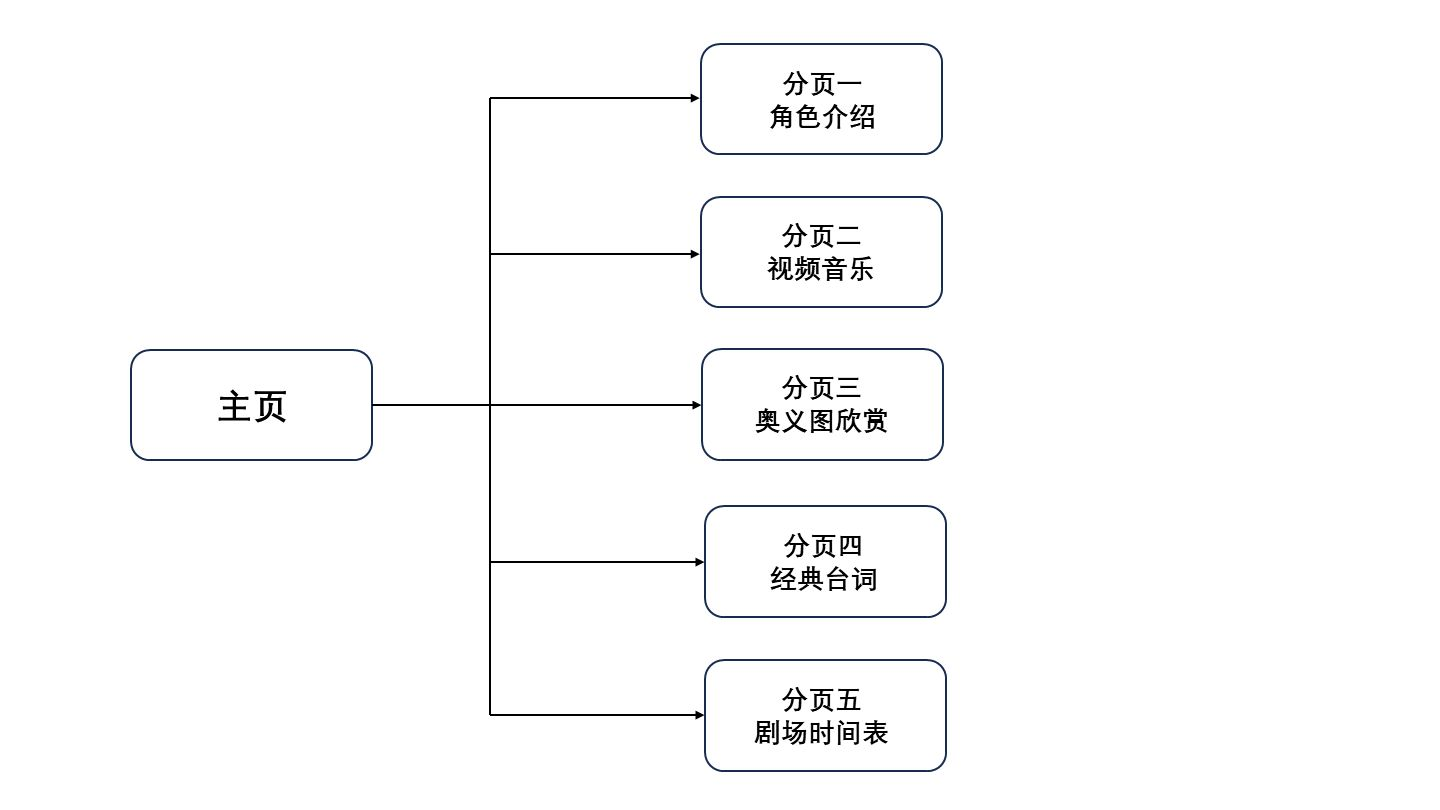
\includegraphics[scale=0.2]{images/1-1.jpg}
	\caption{个人网页整体框架}
	\label{fig1-1}
\end{figure}
具体来说,全部网页主要包含了以下元素:
\begin{enumerate}
	\item 顶部导航栏
	\item 主页:火影简介
	\item 分页面一:角色介绍
	\item 分页面二:视频音乐
	\item 分页面三:奥义图欣赏
	\item 分页面四:经典台词
	\item 分页面五:剧场时间表
	\item 其他:返回寝室主页
\end{enumerate}

\section{个人网页主页设计}

\subsection{导航栏设计}
导航栏在网页设计中扮演着重要的角色,它不仅需要在视觉上与主体内容区分开来,而且要位于页面的顶部,以便用户能够快速访问。为了实现这一目标,我通过CSS对导航栏进行了细致的样式定义,以确保其外观和布局满足设计需求。

以下是我为导航栏设置的CSS样式代码:

\begin{verbatim}
	.nav {
		background-color: #fff;
	}
	.nav li {
		width: 14.2%;
		height: 60px;
		float: left;
		text-align: center;
	}
	.nav li a {
		display: inline-block;
		width: 100%;
		height: 100%;
		font-size: 18px;
		line-height: 60px;
	}
	.nav li a:hover {
		text-decoration: underline;
		color: #fff;
		background-color:#09d2fe;
	}
\end{verbatim}

\newpage
这部分代码实现的作用如下:
\begin{enumerate}[label=\arabic*.]
	\item \textbf{背景颜色:} \texttt{.nav} 的背景颜色被设置为白色(\#fff),这使得导航栏在视觉上清晰,易于阅读。
	\item \textbf{浮动布局:} 通过 \texttt{float: left;},使得列表项(\texttt{li})水平排列
	\item \textbf{文本居中:} \texttt{text-align: center;} 确保了列表项中的文本在水平方向上居中显示。
	\item \textbf{链接样式:} \texttt{.nav li a} 定义了链接的尺寸和字体大小,使得链接覆盖整个列表项区域,便于用户点击。
	\item \textbf{行高与高度一致:} \texttt{line-height: 60px;} 使得文本垂直居中
	\item \textbf{悬停效果:} \texttt{.nav li a:hover} 定义了鼠标悬停在链接上时的视觉效果。文本装饰变为下划线,颜色变为白色,背景颜色变为亮蓝色(\#09d2fe),使用户能够清晰地看到哪个链接是当前被选中的。
	\item \textbf{视觉反馈:} 悬停效果提供了即时的视觉反馈,告诉用户他们的鼠标指针位于哪个链接上
\end{enumerate}

\newpage

\subsection{主页设计}
主页主要包括导航栏和正文内容两部分,导航栏在上文已详细介绍,重点介绍正文部分。正文部分我介绍了火影忍者动漫的相关信息,当鼠标移动到相关模块时会浮现具体人名,在其下方放置了一个宣传视频,在页面最底部放置了几张人物图以充实内容。

\begin{figure}[h]
\centering
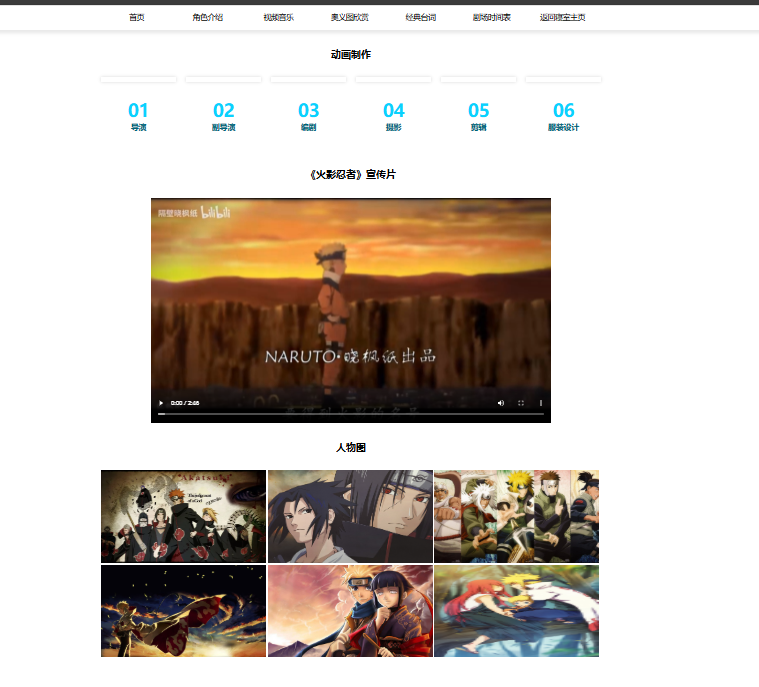
\includegraphics[scale=0.5]{images/2-1.png}
\caption{主页设计}
\label{fig2-1}
\end{figure}
\newpage

\section{分页面设计}
\subsection{页面 1 角色介绍}
在这个部分,我想介绍一下火影忍者中的高人气忍者,于是制作了七个角色卡片,每个卡片包含角色图片和对角色的简要介绍。

\begin{figure}[h]
	\centering
	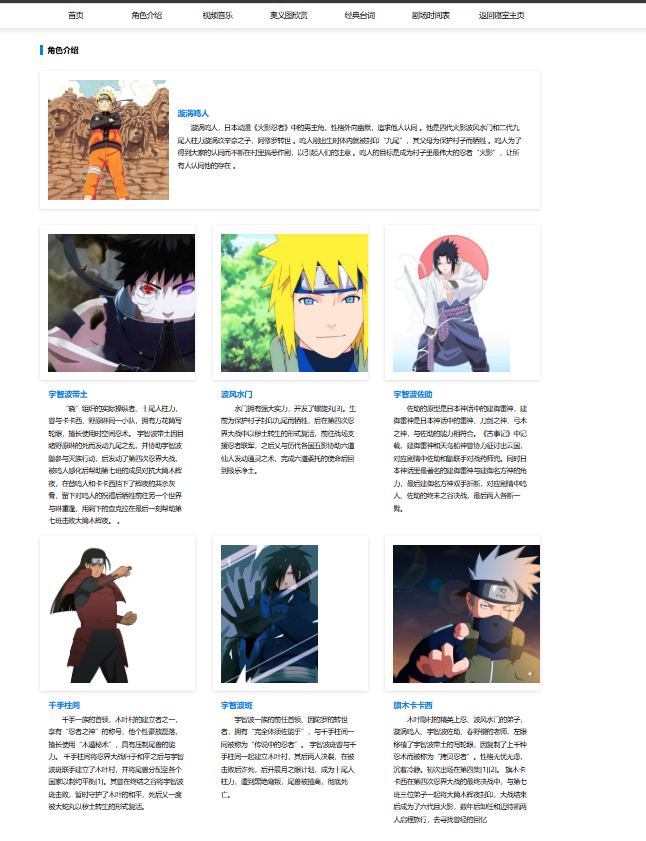
\includegraphics[scale=0.3]{images/2-2.png}
	\caption{分页面 1}
	\label{fig2-2}
\end{figure}


\newpage

\subsection{页面 2 视频音乐}
在这个页面中我放置了一个视频和三首音乐,视频是关于一个人物的特写,音乐则选取了这部动漫中的片头片尾曲和插曲。
\begin{figure}[h]
	\centering
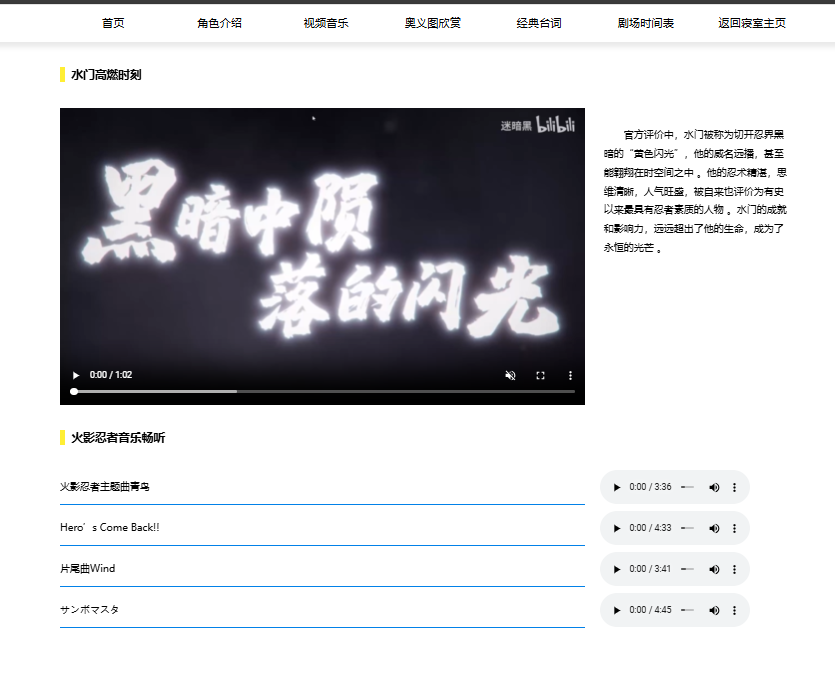
\includegraphics[scale=0.25]{images/2-3.png}
\caption{分页面 2}
\label{fig2-3}
\end{figure}

\newpage

\subsection{页面 3 奥义图欣赏}
在页面三中我选择放置了一些火影忍者中的奥义图,其中许多奥义图都传达出人物的信念与理想。
\begin{figure}[h]
	\centering
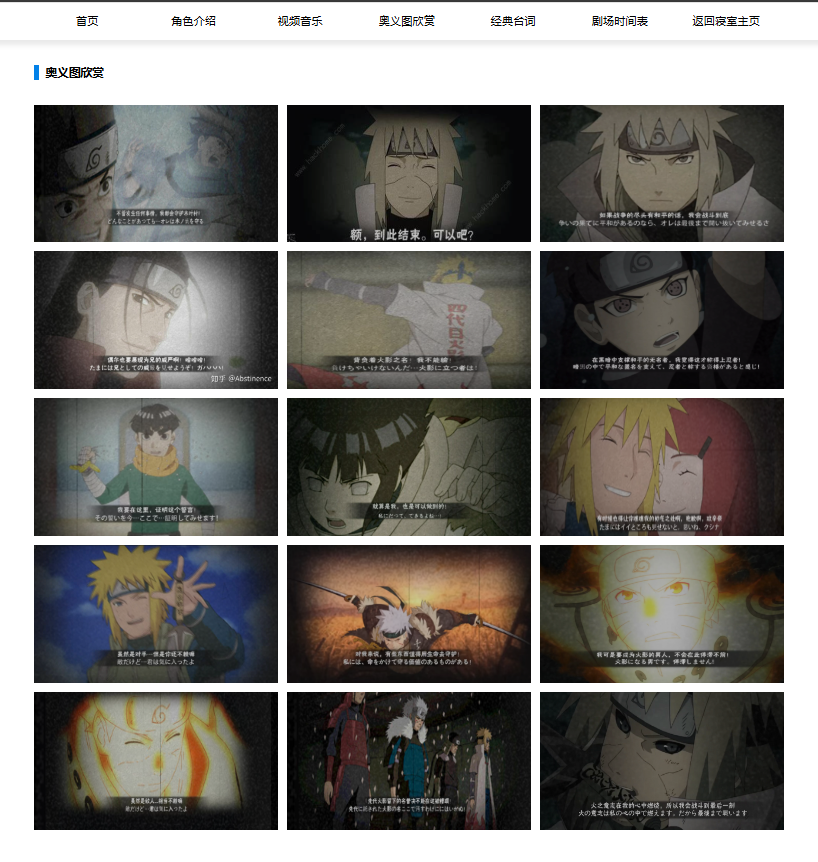
\includegraphics[scale=0.25]{images/2-4.png}
\caption{分页面 3}
\label{fig2-4}
\end{figure}

\newpage

\subsection{页面 4 经典台词}
在这个页面中我选取了火影忍者中一些角色的台词,这些台词给我带来了许多思考与启发。

\begin{figure}[h]
	\centering
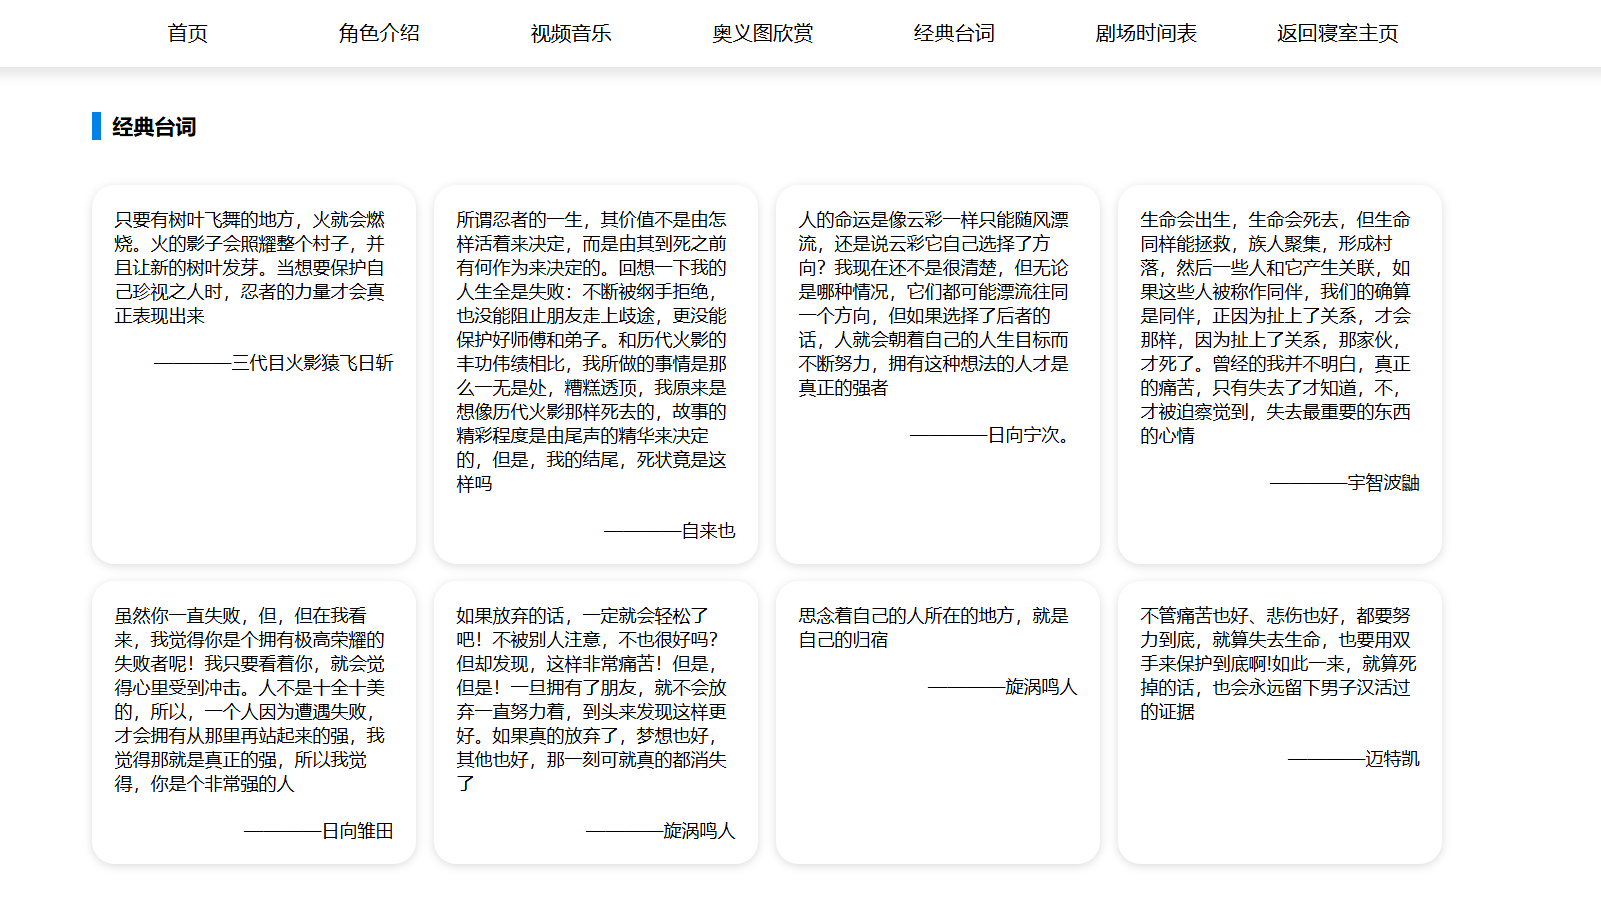
\includegraphics[scale=0.3]{images/2-5.png}
\caption{分页面 4}
\label{fig2-5}
\end{figure}

\newpage

\subsection{页面 5 剧场时间表}
在这个页面中我通过html中的table制作了一个表格,上面枚举了火影忍者上映以来的剧场版电影,如果有同样喜欢火影的可以借此观影。


\begin{figure}[h]
	\centering
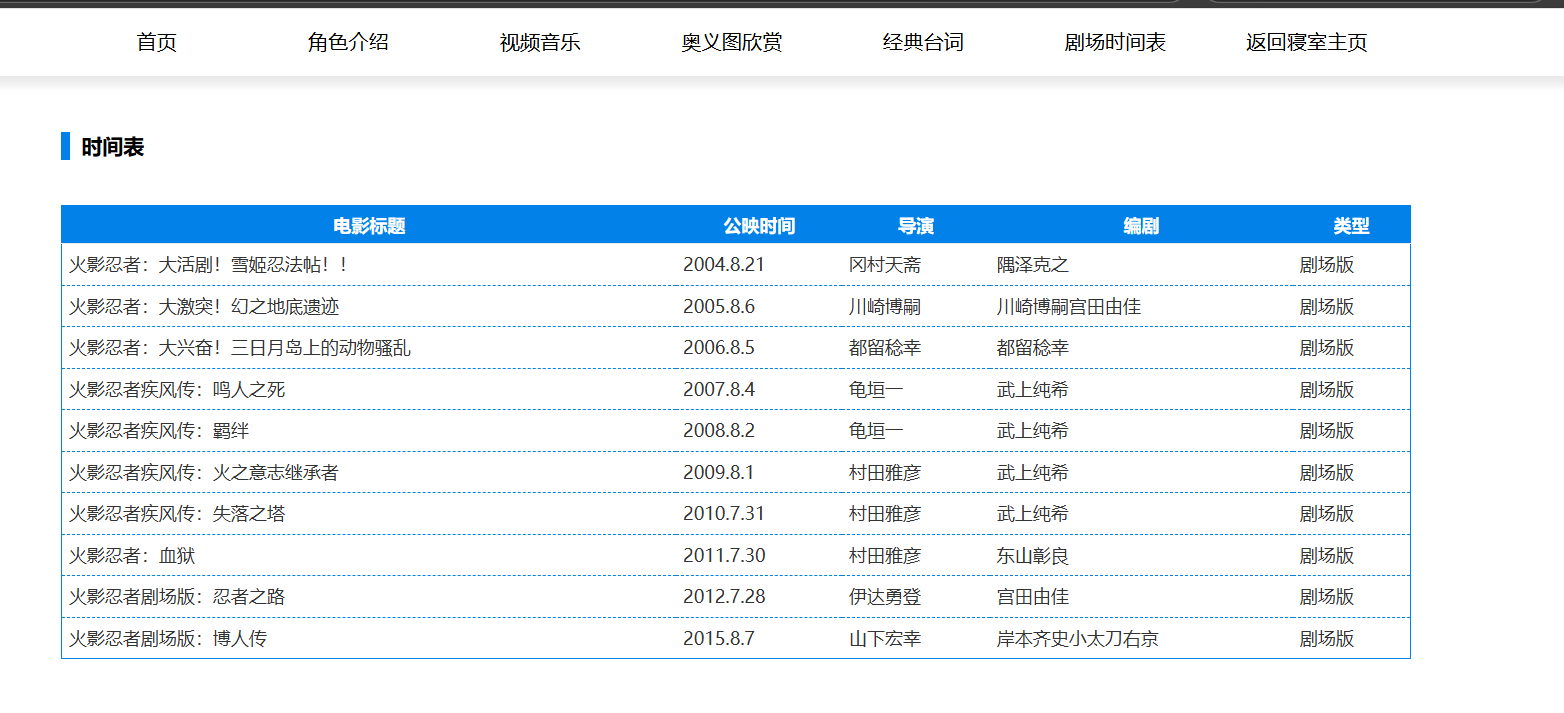
\includegraphics[scale=0.3]{images/2-6.png}
\caption{分页面 5}
\label{fig2-6}
\end{figure}

\newpage

\section{网页设计小结}
通过这次网页设计的经历,我切身体会到了网页设计的魅力。尽管相对于目前互联网上的网站,我设计的web显得尤为幼稚,但是能够将自己喜欢的东西制作成网站确实为我带来不小的成就感。同时,在不断的出错与改正中,我也逐渐熟悉了html语言,感受到他与已学过的py和c的不同。此外,Dreamweaver这一软件大大降低了我这一初学者进行网站设计的难度,其代码补全功能为我带来了不小的便捷。

\section{课程的收获和建议}
\subsection{一点建议}
到最后做大作业的时候才发现之前所学习的知识将在web设计中串联使用,在布置任务的时候可以与前面知识的相串联,可以增强知识的融会性,从而在做最后大作业时更加得心应手。

\subsection{计算机基础知识}
作为一名计算机专业的学生,计算机基础知识对我们来说好比高楼的地基,了解好这些基础的知识有助于我们更好确定未来的方向。

\subsection{文档撰写工具LaTeX}
学习完latex以后,不由得被其工整和美观所深深折服,相信这门强大的工具一定会在我日后的学习生涯中发挥重大的作用。

\subsection{编程工具Python}
相比于c,py是一门更为直接明了的语言,其简洁的代码风格深受我所爱,在课程中深深体会到了高级语言的强大。令人感到愉悦的是,在学习py的过程中并没有觉得与c感到相干涉冲突而混乱,更多的是感受到python的简洁与强大,让我感受到与c语言截然不同的风格,希望以后的课程可以增加python这一部分的内容,让同学们能够学习更多py相关知识。

\subsection{图像设计软件Photoshop}
很遗憾由于时间原因本学期未能学习到ps相关知识。

\subsection{版本管理软件Git}
这节课我学习了Git的基础知识,掌握了基本操作流程,可惜网页制作过程中gitee出现问题无法推送最后只能选择github了。

\subsection{网页制作Dreamweaver}
Dreamweaver的预览和拆分功能能够帮我实时的看到我所设计的web,对于我这样的新生可以说十分的友好了。尽管网页设计的过程中遇到了很多困难,但是看到自己的成品也还是很有成就感的,总体来说还是很有乐趣的。

	
\end{document}
